\newpage
\subsection{Variables aléatoires particulières}

\subsubsection{Schéma de relation entre les variables aléatoires}
\begin{center}
	\begin{tabular}{ccc}
		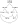
\includegraphics[width=0.5\textwidth]{images/schema_relation_va.pdf}\\
		Schéma de relation entre les différentes variables aléatoires
	\end{tabular}
\end{center}


\newpage
\subsubsection{Variable binomiale$\mathcal{B}(n,p)$}
Une variable binomiale est une expérience avec $n$ répétitions. On veut savoir le nombre $k$ de fois qu'un évènement $A$, de probabilité p, se produit :

\begin{center}
$\begin{array}{llll}
P(V=k)&=\left(\begin{array}{c}n\\k\end{array}\right)&p(\text{obtenir $k$ fois $A$})&p(\text{$n-k$ fois ne pas obtenir $A$})\\
      &=\left(\begin{array}{c}n\\k\end{array}\right)&p^k&(1-p)^{n-k}\\[0.3cm]
      &=\dfrac{n!}{k!(n-k)!}&p^k&(1-p)^{n-k}\\
\end{array}$
\end{center}
La variable $V$ est appelée variable binomiale de paramètre $p$ et d'exposant $n$ et est notée $B(n,p)$. C'est la somme de $n$ de variable indicatrices.


\paragraph{Calcul de la moyenne $E(B(n,p))$}
\begin{align*}
\mu &=\displaystyle\sum_{k=0}^{n} x_ip_i\\
    &=\displaystyle\sum_{k=0}^{n} k \left(\begin{array}{c}n\\k\end{array}\right)p^k(1-p)^{n-k}\\
    &=\displaystyle\sum_{k=1}^{n} \dfrac{n!}{(k-1)!(n-k)!}p^k(1-p)^{n-k}\\
\intertext{On remplace $k-1$ par $l$ :}
    &=\displaystyle\sum_{l=0}^{n-1}  \dfrac{n(n-1)!}{l!(n-l-1)!}p^{l+1}(1-p)^{n-l-1}\\
    &=np\displaystyle\sum_{l=0}^{n-1} \left(\begin{array}{c}n-1\\l\end{array}\right)p^{l}(1-p)^{n-l-1}\\
    &=np(p+(1-p))^{n-1}\\
    &=np\\
\end{align*}

\paragraph{Calcul de la variance $D^2(B(n,p))$}
\paragraph{Calcul de la fonction génératrice $\psi(t)$}
$$\boxed{\psi_x(t) = E(e^{tx}}$$
\begin{align*}
\psi(t) &= \sum_{k=0}^n e^{tk} \left(\begin{array}{c}n\\k\end{array}\right) p^k (1-p)^{n-k}\\
        &= \sum_{k=0}^n \left(\begin{array}{c}n\\k\end{array}\right) (e^tp)^k(1-p)^{n-k}\\
        &= ((1-p)+e^tp)^n\\
        &=(pe^t+(1-p))^n\\
\end{align*}

\paragraph{Calcul de la moyenne $E(B(n,p))$ via la fonction génératrice $\psi(t)$}
$$\boxed{\psi_x(t) = (pe^t+(1-p))^n}$$
\begin{align*}
E(X) &= \psi_x(t)|_{t=0}\\
     &= ( e^tp + (1-p))^n|_{t=0}\\
     &= n ( e^tp + (1-p) )^{n-1}e^tp&\text{pour } t=0\\
     &= n ( p + 1 - p )^{n-1} p\\
     &= np\\
\end{align*}

\paragraph{Calcul de la variance $D^2(B(n,p))$ via la fonction génératrice $\psi(t)$}


\paragraph{Calcul de la stabilité}



\newpage
\subsubsection{Variable de Poisson $\mathcal{P}_\lambda$}
Une variable de poisson est uniquement une binomiale dont la répétition $n$ est "grand" ($n\geq30$) et que la probabilité $p$ est "petit" ($p\leq0,1$).

\begin{center}
$\begin{array}{lll}
P(V=k)&=\left(\begin{array}{c}n\\k\end{array}\right)&p^k(1-p)^{n-k}\\[0.3cm]
      &=\dfrac{n!}{k!(n-k)!}&p^k(1-p)^{n-k}\\[0.3cm]
      &=\dfrac{1}{k!}n(n-1)(n-2)\dots(n-k-1)&p^k(1-p)^{n-k}\\[0.3cm]
      &=\dfrac{1}{k!}n^k\left(1-\dfrac{1}{n}\right)\left(1-\dfrac{2}{n}\right)\dots\left(1-\dfrac{k-1}{n}\right)&p^k(1-p)^{n-k}\\[0.3cm]
      &=\dfrac{1}{k!}n^k\left(1-\dfrac{1}{n}\right)\left(1-\dfrac{2}{n}\right)\dots\left(1-\dfrac{k-1}{n}\right)&\dfrac{p^k\left(1-p\right)^{n}}{(1-p)^k}\\[0.3cm]
      &=\dfrac{1}{k!}n^k\left(1-\dfrac{1}{n}\right)\left(1-\dfrac{2}{n}\right)\dots\left(1-\dfrac{k-1}{n}\right)&\dfrac{p^k\left(1-\dfrac{np}{n}\right)^{n}}{(1-p)^k}\\[0.3cm]
\end{array}$
\end{center}
Sous une autre forme :
\begin{center}
$\begin{array}{llcl}
P(V=k)&=\dfrac{n^kp^k}{k!}&\left(1-\dfrac{np}{n}\right)^n&\dfrac{\left(1-\dfrac{1}{n}\right)\left(1-\dfrac{2}{n}\right)\dots\left(1-\dfrac{k-1}{n}\right)}{(1-p)^k}\\[0.3cm]
&=\dfrac{(np)^k}{k!}&e^{-\lambda}&\dfrac{\left(1-\dfrac{1}{n}\right)\left(1-\dfrac{2}{n}\right)\dots\left(1-\dfrac{k-1}{n}\right)}{(1-p)^k}\\[0.3cm]
\end{array}$
\end{center}
Et donc quand $n\rightarrow\infty$ :
\begin{center}
$P(V=k)\stackrel{n\rightarrow\infty}{=}\dfrac{\lambda^k}{k!}e^{-\lambda}\dfrac{(1-1)(1-1)\dots(1-1)}{(1-p)^k}$
\end{center}
$$\boxed{P(V=k)\stackrel{n\rightarrow\infty}{=}\dfrac{\lambda^k}{k!}e^{-\lambda}=P_\lambda}$$


\paragraph{Calcul de la moyenne $E(P_\lambda)$}
\begin{center}
$\begin{array}{ll}
\mu&=\displaystyle\sum_{k=0}^{\infty}x_ip_i\\
&=\displaystyle\sum_{k=0}^{\infty}k\dfrac{\lambda^k}{k!}e^{-\lambda}\\
&=\displaystyle\sum_{k=0}^{\infty}\dfrac{\lambda^{k-1}\lambda}{(k-1)!}e^{-\lambda}\\
&=\displaystyle\lambda e^{-\lambda}\sum_{k=0}^{\infty}\dfrac{\lambda^{k-1}}{(k-1)!}\\
&=\displaystyle\lambda e^{-\lambda}e^{\lambda}\\
&=\lambda
\end{array}$
\end{center}


\paragraph{Calcul de la variance $D^2(P_\lambda)$}
\begin{align*}
\sigma^2&=\displaystyle\sum_{k=0}^{\infty}x_i^2p_i-\mu^2\\
&=\displaystyle\sum_{k=0}^{\infty}k^2\dfrac{\lambda^k}{k!}e^{-\lambda}-\mu^2\\
\intertext{On remplace $k^2$ par $k(k-1)+k$}
&=\displaystyle\sum_{k=0}^{\infty}k(k-1)\dfrac{\lambda^k}{k!}e^{-\lambda}+\sum_{k=0}^{\infty}k\dfrac{\lambda^k}{k!}e^{-\lambda}-\mu^2\\
&=\displaystyle\sum_{k=0}^{\infty}k(k-1)\dfrac{\lambda^k}{k!}e^{-\lambda}+\mu-\mu^2\\
&=\displaystyle\sum_{k=0}^{\infty}k(k-1)\dfrac{\lambda^{k-2}\lambda^2}{k(k-1)(k-2)!}e^{-\lambda}+\mu-\mu^2\\
&=\displaystyle\lambda^2e^{-\lambda}\sum_{k=0}^{\infty}\dfrac{\lambda^{k-2}}{(k-2)!}+\mu-\mu^2\\
&=\displaystyle\lambda^2e^{-\lambda}e^\lambda+\mu-\mu^2\\
&=\displaystyle\lambda^2+\lambda-\lambda^2\\
&=\lambda
\end{align*}



\paragraph{Calcul de la fonction génératrice $\psi(t)$}
\begin{align*}
(t)&=\displaystyle\sum_{k=0}^{\infty}e^{tk}e^{-\lambda}\dfrac{\lambda^k}{k!}\\
&=e^{-\lambda}\sum_{k=0}^{\infty}\dfrac{(\lambda e^t)^k}{k!}\\
&=e^{-\lambda}e^{\lambda e^t}\\
&=e^{\lambda(e^t-1)}\\
\end{align*}



\paragraph{Calcul de la stabilité}
\begin{align*}
\psi_{1+2}(t)&=\psi_1(t)\psi_2(t)\\
&=e^{\lambda_1(e^t-1)}e^{\lambda_2(e^t-1)}\\
&=e^{\lambda_1(e^t-1)(\lambda_1+\lambda_2)}\\
\end{align*}
La variable est bien stable.






\newpage
\subsubsection{Variable exponentielle négative}
\subsubsection{Variable Normale $\mathcal{N}(\mu,\sigma)$}


\paragraph{Propriété d'opposé}\label{propriete-normale-oppose}
Soit $\bar{X_1}$ et $\bar{X_2}$ deux variables normales. Si $\bar{X_2}$ est l'opposé de $\bar{X_1}$ ( $\bar{X_2}$ = -$\bar{X_1}$ ) alors
\begin{center}
$\boxed{\bar{X}_1 \sim N \left( \mu_1, \sigma \right)$ et $\bar{X}_2 \sim N \left( -\mu_2, \sigma \right)}$
\end{center}




\paragraph{Propriété d'addition}\label{propriete-normale-addition}
Soit $N(\mu_1,\sigma_1)$ et $N(\mu_2,\sigma_2)$ deux variables normales indépendantes et $\psi_1(t)$ et $\psi_2(t)$ leurs fonctions génératrices.
\begin{center}
$\begin{array}{LL}
\psi(t) &= \psi_1(t).\psi_2(t)\\
        &= e^{\mu_1+t+\sigma_1^2t^2/2}.e^{\mu_2+t+\sigma_2^2t^2\frac{1}{2}}\\
        &= e^{(\mu_1+\mu_2)t+\frac{1}{2}(\sigma_1^2+\sigma_2^2)t^2}\\
\end{array}$
\end{center}
On obtient bien une fonction génératrice d'une normale de paramètres $(\mu_1+\mu_2)$ et $\sqrt{\sigma_1^2+\sigma_2^2}$.
$$\boxed{N(\mu_1,\sigma_1) + N(\mu_2,\sigma_2) = N\left(\mu_1+\mu_2,\sqrt{\sigma_1^2+\sigma_2^2}\right)}$$



\subsubsection{Variable Khi$^2$}
\subsubsection{Variable Student $t_n$}
\label{propriete-student}
\subsubsection{Variable Snedecor $\mathcal{F}_{(m,n)}$}


